\documentclass[tikz,border=2pt]{standalone}
\usepackage{amsmath,amssymb}
\usepackage{tikz}

\begin{document}
% Holding cost over one EOQ cycle: h times the area under the stock curve (a triangle of
% area y t0 / 2), i.e. h y/2 per unit time since the average stock is y/2.
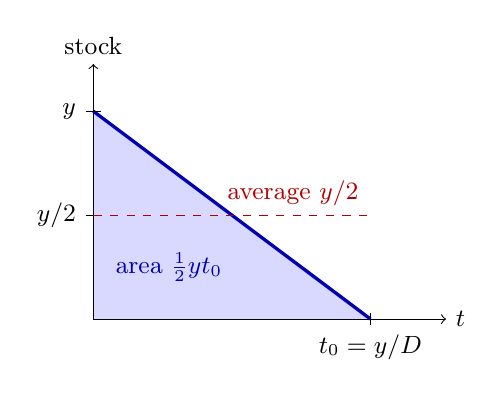
\begin{tikzpicture}[every node/.style={font=\small}, x=0.32cm, y=0.12cm]
	\fill[blue!15] (0,0) -- (0,22) -- (11,0) -- cycle;
	\draw[->] (0,0) -- (14,0) node[right] {$t$};
	\draw[->] (0,0) -- (0,27) node[above] {stock};
	\draw[blue!70!black, very thick] (0,22) -- (11,0);
	\draw (0.3,22) -- (-0.3,22) node[left] {$y$};
	\draw (0.3,11) -- (-0.3,11) node[left] {$y/2$};
	\draw (11,0.6) -- (11,-0.6) node[below] {$t_0=y/D$};
	\draw[red!70!black, dashed] (0,11) -- (11,11) node[pos=0.72, above] {average $y/2$};
	\node[blue!70!black] at (3.0,5.5) {area $\tfrac12yt_0$};
\end{tikzpicture}
\end{document}
